\documentclass[12pt]{report}

\usepackage[utf8]{inputenc}
\usepackage{listings}
\usepackage{algpseudocode}	   % pseudo code
\usepackage{graphicx}		       % graphics
\usepackage{amsmath}		       % math symbols
\usepackage{amssymb}		       % math symbols
\usepackage[colorlinks,        % hyperlinks
            linktocpage,
            linkcolor=black,
            urlcolor=black]
            {hyperref}

\graphicspath{{installImages/}}

% COMMANDS
% ----------------------------------------------------------------
\newcommand{\answer}{\textbf{A:}}
\newcommand{\TITLE}{\Large\textbf{DBS:} Exercise 1}
\newcommand{\AUTHOR}{\normalsize{John Nguyen, Gavithishan Ravechandran}}
\newcommand{\TUTOR}{\normalsize{Felicia Burtscher (Thur 12pm)}}

% DOCUMENT
% ----------------------------------------------------------------
\begin{document}
\noindent\TITLE \hfill 28/4/17\\[3pt]
\TUTOR\\
\AUTHOR\\
\rule{\textwidth}{0.4pt}\\}

\section*{1. Aufgabe: Begriffe \& Definitionen}

\begin{enumerate}
\item[(4 P)] Was ist ein Datenbanksystem? Wie stehen die Begriffe Datenbank, Datenbanksystem und Datenbankmanagementsystem zueinander im Verhältnis?
\item[\answer]
  Eine Datenbank (DB) ist eine Sammlung von verwandten Daten und ein Database-Management-System (DBMS) ist ein allgemeines Software-System, das die Herstellung und Verwaltung einer Datenbank verwendet wird. Die Zusammenfassung einer DB und eines DBMSs wird ein Datenbanksystem (DBS) genannt.

  % A Database (DB) is a collection of related data and a Database Management System (DBMS) is a general purpose software system used to create and maintain a DB. A DB together with a DBMS is called a Database System (DBS).

\item[(6 P)] Aus welchen Teilen setzt sich ein Datenmodell zusammen? Welche Funktion erfüllen die Teile
\item[\answer]
  Das Datenmodell beschreibt die darunterliegende Struktur einer Datenbank. Es ist eine Sprache, die aus dem Data-Definition-Language (DDL) und dem Data-Manipulation-Language (DML) besteht. Der DDL bietet Methoden sowohl zur Beschreibung des Datenbankschemas (z.B. welche Datentypen und Verhältnisse die Daten besitzen) als auch zusätzliche Attribute wie Beschränkungen. Der DML ermöglicht den Zugang und Manipulierung der Daten, indem Methoden zum Einfügen, Abfragen, Updaten und Löschen definiert werden.

  % The data model describes the underlying structure of a DB. Formally it is a language, composed of a Data-Definition-Language (DDL) and a Data-Manipulation-Language (DML). The DDL provides a way to specify the DB Schema (such as specifying data types and relationships) as well as defining additional properties on the data such as constraints. The DML is used to to access and manipulate data in the DB. It defines techniques to insert, retrieve, update and delete data items.

\item[(5 P)] Was versteht man unter "physischer Datenunabhängigkeit"?
\item[\answer]
  Physische Datenunabhängigkeit ist eine Art von Datenabstraktion, wobei komplexe Implementierungen auf der physischen Ebene (d.h. \textit{wie} die Daten gespeichert werden) vom Benutzer der logischen Ebene verborgen werden, der hauptsächlich nur mit den konzeptionellen Datenstrukturen befasst. Ein Anwendungsprogramm besitzt physische Datenunabhängigkeit, falls sie immer noch valide bleibt, obwohl die Speicherstruktur geändert hat.

  % Physical data independence is a form of data abstraction, whereby possibly complex implementations of \textit{how} the data is stored in the physical level is hidden from users of the logical level, who are only concerned with the simple description of \textit{conceptual} structure of the data. An application program has physical data independence when it does not depend on the physical implementation of the data structures, and thus are still valid when the storage structure is changed.

\item[(5 P)] Was versteht man unter "logischer Datenunabhängigkeit"?
\item[\answer]
  Obwohl die Daten auf der logischen Ebene wesentlich einfacher dargestellt werden, bleibt immer noch einige Komplexitäten. Dadurch ist logische Datenunabhängigkeit die höchste Abstraktionsebene, in der die Benutzer einen möglichst einfacher Ausblick (d.h. die semantische Bedeutung) der Daten bekommen. Damit bleiben Anwendungsprogramme immer noch valide, auch wenn das Schema (auf der logischen Ebene) sich verändert hat.

  % Although the representation of data on the logical level is simpler than on the physical level, logical data independence exist to hide the remaining complexities. It is the highest level of abstraction and provides the simplest view of the data for users concerned with the \textit{content} inherent in the data. Application programs inhibit logical data independence when they remain valid after changes to the schema of the DB.

\item[(4 P)] Nennen Sie zwei funktionale und zwei nicht-funktionale Anforderungen an ein Datenbanksystem.
\item[\answer]
  Zwei funktionale Anforderungen einer DB sind: 1) sie muss sicher sein, d.h. einige Daten kann nur von berechtigten Personen greifbar sein), und 2) sie muss konsistent sein, d.h. verschiedene Exemplare von Daten müssen übereinstimmen.

  Zwei nicht-funktionale Anforderungen sind: 3) Die DB soll möglichst benutzerfreundlich aufgebaut werden, und 4) sie muss möglichst effizient laufen, d.h. schnelle Antwort- und Updatezeit.

  % Two functional requirements of a DB are 1) that it must be secure (data can only be accessed by users authorized to do so), and 2) it must be consistent (multiple instances of a data item contain the same content). Two non-functional requirements include 3) the DB must be user friendly, and 4) it is efficient (fast access and modification of data).

\item[(1 P)] Was sind Meta-Daten?
\item[\answer]
  Metadaten sind Daten, die sowohl die Struktur der DB als auch den Typ und Format jedes Datenobjektes beschreiben. Außerdem kann die Metadaten Beschränkungen der Daten bestimmen. Die Metadaten werden (gentrennt von der DB-Daten) im DB-Catalog gespeichtert.

  % Meta-data is data used to describe the DB in terms of its structure as well as the type and format of each data item. Additionally it includes constraints on the data. The Meta-data is stored in the DB Catalog, which is kept separate from the data in the DB.

\end{enumerate}

\section*{2. Aufgabe: Arten von Datenbanksysteme}

\begin{enumerate}
\item[(5 P)] Recherechieren Sie, welche Arten von Datenbanksystemen existieren und wie sich diese gruppieren lassen.
\item[\answer]
  Es gibt drei grundlegende Arten von DBSs, welche sich von ihrer technischen Umsetzung unterscheiden.\\

  \textbf{1. Hierarchie Modell, Netzwerk Modell}. Das Hierarchie Modell wird nach einer nach unten gerichteten Baumstruktur aufgebaut. Die Beziehung zwischen den Daten wird mit Pfeilen dargestellt. Das Netzwerk Modell entspricht zum größten den Hierarchischen Modell, aber bei diesem Modell können die Daten untereinander verbunden werden. Somit entspricht es nicht immer der nach unten gerichteten Baumstruktur.\\

  \textbf{2. Relationales Modell, Deduktives Modell}. Das relationales Modell wird nicht wie die beiden oberen Modellen in einer Baumstruktur gespeichert, sondern in einer zweidimensionalen Tabelle. Die Bearbeitung der Daten erfolgt auf mathematischer Relationstheorien. Das Deduktives Modell entspricht dem relationalen Modell, nur dassdie Daten auf Prädikats Berechnungen bearbeitet werden.\\

  \textbf{3. Entity-Relationship Modell, Objekt-orientiertes Modell}. Das Entity-Relationship Modell stellt die Daten (Entities) und ihre Beziehungen (Relationships) zueinander als Objekte dar. Das objekt-orientiertes Modell erweitert dieses Konzept, indem Operationen auf den Daten ermöglicht werden. Damit entsprechen Daten-Objekte den Klassen vom Objekt-Orientierte-Paradigma.

  % The main types of DBSs: \textit{Relational, Deductive, Entity-Relationship, Object-Oriented, Hierarchical} and \textit{Network}.\\\\
  % \textbf{Relational} DBSs use collections of tables to represent data and the relationships between those data.\\\\
  % The \textbf{deductive} DBS is extends the relational model by allowing additional data to be deduced using predicates on the stored data.\\\\
  % The \textbf{Entity-Relationship} (ER) model represents data as objects (entities) and expresses relationships between these objects.\\\\
  % The \textbf{Object-oriented} (OO) model extends the ER model by incorporating object-oriented design principles into the DB such as adding operations to data objects.\\\\
  % \textbf{Hierarchical} DBSs employ a parent-child-tree model to structure its data.\\\\
  % The \textbf{Network} model is similar to the Hierarchical model in that it also uses a tree structure, however with many-parent-many-child relationships.
  % \\\\
  % We can generally group these systems as 1) Relational, Deductive, 2) ER, OO, 3) Hierarchical, Network

\item[(5 P)] Was sind NoSQL-Datenbanksysteme? Welche Arten von Datenbanksystemen könnten NoSQL-Datenbanksysteme sein. Begründen Sie Ihre Antwort.
\item[\answer]
NoSQL ist eine Abkürzung für \textit{Not Only SQL}. Der Vorteil von NoSQL-Datenbanksystemen sind, dass sie große Mengen an Daten speichern können und abrufen können und damit sind sie geeignet für Big-Data/Data-Mining Anwendungen. Dies wird ermöglicht, da sie nicht der relationalen Ansatz verfolgen oder keine festen Tabellenschemas verfolgen. Oft sind die Schemas dynamisch, sodass die DB mit sich ständig verändernd Daten umgehen kann.

Da NoSQL-Datenbanksysteme nicht den relationalen Ansichten verfolgen, gehören alle andern Arten der Datenbanken zu der NoSQL-Datenbanksystemen. Es wird immer nur die erste Instanz betrachtet, so können zum Beispiel nur Daten direkt angelegt werden(nicht relational) aber die Daten selbst intern entsprechen der relationalen Modellen.

% NoSQL DBSs were developed to be able to manage huge data sets containing non data not suitable to RDBMSs (such as data generated by social media websites: posts, comments, likes). NoSQL DBs are used for Big-Data/Data-Mining applications. The data is generally modelled in ways other the table structures of relational DBs and vary greatly (key-value, document, graph based data stores). Furthermore, the schemas of NoSQL DBs are typically dynamic to accomodate for rapidly changing data structures, and can be updated without service interruptions. NoSQL DBSs are simply alternatives to relational DBs and encompass a wide range of DB types. Thus they can be exhibit traits of ER, OO as well as hierarchical DBs.

\item[(10 P)] Was ist RDF? Erklären Sie kurz den Aufbau, bzw. die Funktionsweise von RDF. Geben Sie einen einfachen Beispieldatensatz in RDF an.
\item[\answer]
  Der \textbf{Resource Description Framework} (RDF) ist eine Sammlung von Spezifikationen des World-Wide-Web-Consortiums (W3C) zur Verarbeitung der Metadaten von Webressourcen. Eine Ressource ist alles, was mit einem Uniform-Resource-Identifier (URI) identifiziert werden kann, wie z.B ein Dokument oder datei. Der RDF begründet ein allgemeines System zur Beschreibung solche Ressourcen, ohne Details des Anwendungsbereich anzunehmen.\\

  Das RDF-Datenmodell wird durch Aussagen aufgebaut, die aus drei Komponenten bestehen. Die erste Komponente ist das Subjekt (eine Ressource), zweitens kommt der Property-Type (ein Attribute des Subjekts), und zuletzt ist der Wert (eine andere Ressource oder ein atomarer Wert, z.B String oder Zahl). Der Property-Typ verknüpft die äußeren Kompoonenten. Zum Beispiel, die Aussage

  \begin{center}
    (resource R) --- property type P $\rightarrow$ (value V)
  \end{center}

  bedeutet, dass die Ressource R den Wert V für das Attribut P hat. In diesem Modell kann die Ressourcen und Werte als Knoten und die Property-Types als Kanten eines gerichteten Graphen betrachtet werden. Wir zusammenfassen die Aussage als 3-Tupel.\\

  Als ein konkretes Beispiel betrachten wir den Datensatz von Studierenden:

  \begin{center}
    \begin{tabular}{l l l l}
      \textbf{student} & \textbf{name} & \textbf{number} & \textbf{major} \\
      \hline
      student1 & bob & 12345 & Comp Sci \\
      student2 & jane & 54321 & Philosophy\\
      ... & ... & ... & ...
    \end{tabular}
  \end{center}

  Im RDF-Format sieht die Daten wie folgt aus:

  \begin{center}
    \begin{tabular}{ l l l l l }
      \{ & student1, & name, & bob & \}\\
      \{ & student1, & number, & 12345 & \}\\
      \{ & student1, & major, & Comp Sci & \}\\
      \{ & student2, & name, & jane & \}\\
      \{ & student2, & number, & 54321 & \}\\
      \{ & student2, & major, & Philosophy & \}\\
      \{ & ... & ... & ... & \}
    \end{tabular}
  \end{center}

  % The \textbf{Resource Description Framework} (RDF) is a collection of specifications from the World Wide Web Consortium (W3C) for the purpose of processing metadata of web resources. A web resource is anything that can be identified by a Uniform Resource Identifier (URI), such as a document or file. Metadata can be used, for example, by a search engine to help discover such resources. The RDF establishes a general system for describing these resources without making assumptions the metadata is being used for. Informally, the RDF data model consists of statements involving a `subject', an `object/value', and an `attribute' relating the subject and the object/value.
  %
  % Formally, the subject represents a resource, the object/value represents either a resource or an atomic value (such as a text string or a number), and the attribute represents a property type. In this data model, the resources and values are nodes in a label directed graph, and the attributes relating them are the edges connecting the nodes. Thus
  %
  % \begin{center}
  %   (resource R) --- property type P $\rightarrow$ (value V)
  % \end{center}
  %
  % states that V is the value of the property type P for resource R. These statements are concretely expressed as 3-Tuples in the form \textit{\{Resource, Property Type, Value\}}. As a concrete example, consider the dataset of students with the following table:
  %
  % \begin{center}
  %   \begin{tabular}{l l l l}
  %     \textbf{student} & \textbf{name} & \textbf{number} & \textbf{major} \\
  %     \hline
  %     student1 & bob & 12345 & Comp Sci \\
  %     student2 & jane & 54321 & Philosophy\\
  %     ... & ... & ... & ...
  %   \end{tabular}
  % \end{center}
  %
  % This table is represented using the RDF format as follows:
  %
  % \begin{center}
  %   \begin{tabular}{ l l l l l }
  %     \{ & student1, & name, & bob & \}\\
  %     \{ & student1, & number, & 12345 & \}\\
  %     \{ & student1, & major, & Comp Sci & \}\\
  %     \{ & student2, & name, & jane & \}\\
  %     \{ & student2, & number, & 54321 & \}\\
  %     \{ & student2, & major, & Philosophy & \}\\
  %     \{ & ... & ... & ... & \}
  %   \end{tabular}
  % \end{center}


\item[(5 P)] Wie könnte eine einfache SPARQL-Abfrage an Ihren Beispieldatensatz aussehen? Erklären Sie, wie ihre Abfrage funktioniert.
\item[\answer]
  Unsere einfache SPARQL Abfrage ersucht die Studentnummern aller Studierende, deren Name gleich `bob' ist und außerdem hat das Hauptfach `Comp Sci':

  % Our simple SPARQL query asks for the student numbers for all students whose name is bob and whose major is Comp Sci:

  \begin{lstlisting}
    PREFIX info: <http://www.example.com/attributeNames/>

    SELECT ?student  ?number

    WHERE {
        ?student  info:name "bob"
        ?student  info:major "Comp Sci"
        ?student  info:number ?number
    }
  \end{lstlisting}

  Zuerst schauen wir die SELECT-Klausel an. Hier deklarieren wir drei Variablen, in denen die Ergebnisse gespeichert werden. Zunächst betrachten wir die WHERE-Klausel. Wir listen die Abfragebedingung als 3-Tupel auf. Jede Bedingung wird auf die Ergebnisse der vorgegangenen Bedingung getestet. Das erste 3-Tupel fragt alle Studierende an, bei denen das \textit{name}-Attribut den Wert `bob' hat. Von denen ersucht das nächste 3-Tupel die Studierende, die `Comp Sci' als Hauptfach studieren. Schließlich bittet das letzte 3-Tupel um die Studentnummern von diesen Ergebnissen.\\

  Zuletzt merken wir, dass in SPARQL, die Attributnamen mittels eines URI bezeichnet werden, wie z.B: http://www.example.com/attributeNames/major. Da jedes Attribut ein gemeinsames (in unserem Beispiel) Präfix haben, können wir dieses in einer Variable speichern, die \textit{info} heißt. Dies wird in der ersten Zeile der Abfrage deklariert.

  % First we will examine the SELECT clause. Here we declare three variables to store the results we wish to receive. Next we turn our attention to the WHERE clause. Here we list our query conditions in the form of 3-Tuples. Each condition will be tested on the results return by the previous condition. The first 3-Tuple requests all students whose \textit{name} attribute has the value `bob'. Of these students, we then request those whose \textit{major} attribute has the value `Comp Sci'. Finally the last 3-Tuple asks for the student number of these results.\\\\
  % Finally we note that in SPARQL, the attribute names must be indicated using a URI, for example: http://www.example.com/attributeNames/major. Since each attribute name shares the same prefix, we can store this prefix in a variable called \textit{info}. This is declared on the first line of the query.

\end{enumerate}

\newpage

\section*{3. Aufgabe: Typische Abfragen}

\begin{enumerate}
\item[(2 P)] Wie könnte umgangssprachlich eine typische Abfrage an ein Datenbanksystem eines Kursverwaltungssystems wie dem KVV aussehen?
\item[\answer]
  Return the all the course information for computer science modules available this semester.

\item[(2 P)] Wie könnte umgangssprachlich eine typische Abfrage an ein Datenbanksystem einer Online-Videothek/Online-Mediathek aussehen?
\item[\answer]
  Return all videos that have the tag 'computer science' in order most views to least views

\item[(2 P)] Wie könnte umgangssprachlich eine typische Abfrage an ein Datenbanksystem einer Photo-Sharing-Plattform wie Instagram aussehen?
\item[\answer]
  Return all photos with the hashtag \textit{\#cat} orderd from newest to oldest.

\item[(2 P)] Wie könnte umgangssprachlich eine typische Abfrage an ein Datenbanksystem eines Mikrobloggingdienstes wie Twitter aussehen?
\item[\answer]
  Return all tweets posted by users who are followed by the user `snoopy'.

\item[(2 P)] Wie könnte umgangssprachlich eine typische Abfrage an ein Datenbanksystem eines sozialen Netzwerks wie Facebook aussehen?
\item[\answer]
  Return usernames of users who have a mutual friend with the user `leonard943'.
\end{enumerate}

\newpage

\section*{4. Aufgabe: PostgreSQL \& Programmiersprachen}

\vspace{1cm}
The following screenshots show the results of the following unix command:
\begin{verbatim}
  apt list --installed
\end{verbatim}
\begin{enumerate}
  \item [INSTALLATION]
  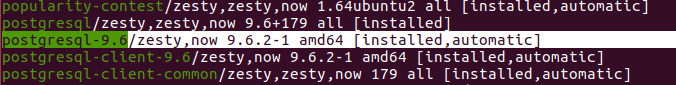
\includegraphics[scale = 0.5]{postgres}\\
  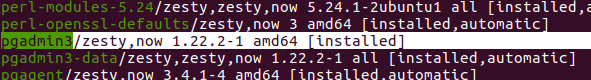
\includegraphics[scale = 0.5]{pgadmin}\\
  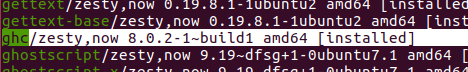
\includegraphics[scale = 0.5]{haskell}\\
  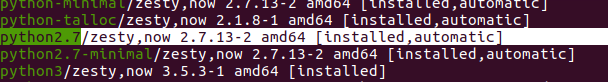
\includegraphics[scale = 0.5]{python}\\
  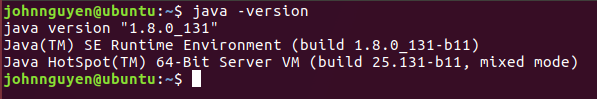
\includegraphics[scale = 0.5]{java}\\

  \item [HASKELL]
  \begin{lstlisting}[language = Haskell]
    main = do
      -- ask for input
      putStrLn "Hey what's your name?"
      -- read input
      name <- getLine
      -- print output
      putStrLn ("Hello " ++ name ++ "!")
  \end{lstlisting}

  This program is executed with the command:
  \begin{verbatim}
    ghc hello.hs && ./hello
  \end{verbatim}
  \vspace{1.5cm}

  \item [PYTHON]
  \begin{lstlisting}[language = Python]
    # prompt for name
    name = raw_input("Hey what's your name? ")
    # print message
    print "Hello " + name + "!"
  \end{lstlisting}

  This program is executed with the command:
  \begin{verbatim}
    python hello.py
  \end{verbatim}
  \vspace{1.5cm}

  \item [JAVA]
  \begin{lstlisting}[language = Java]
    import java.util.Scanner;

    public class Hello {

        public static void main(String[] args) {
            // scanner to read input
            Scanner scanner = new Scanner(System.in);
            // prompt user for name
            System.out.print("Hey what's your name? ");
            // get input
            String name = scanner.next();
            // print message
            System.out.println("Hello " + name + "!");
        }
    }
  \end{lstlisting}

  This program is executed with the command:
  \begin{verbatim}
    javac Hello.java && java Hello
  \end{verbatim}
\end{enumerate}

% \section*{4. Aufgabe: PostgreSQL \& Programmiersprachen}
%
% Bevor Sie mit dieser Aufgabe beginnen empfiehlt es sich eine virtuelle Maschine (kurz VM), wie zum Beispiel "Virtual Box", mit einer aktuellen Linux Version (wie zum Beispiel Ubuntu 16.04 LTS) aufzusetzen, bzw. auf einem eigenen Rechner zu installieren.\\
% \\
% Hinweis: Für alle folgenden Aufgaben in diesem Semester werden wir immer von einer Standard Ubuntu 16.04 Installation ausgehen. Die Software "Virtual Box" und "Ubuntu 16.04 LTS" können kostenfrei aus dem Internet bezogen werden.
%
% \subsection*{PostgreSQL}
%
% \begin{enumerate}
% \item[(5 P)] Installieren Sie PostgreSQL.
% \item[(5 P)] Installieren Sie PgAdmin.
% \end{enumerate}
%
% \newpage
%
% \subsection*{Haskell}
%
% \begin{enumerate}
% \item[(1 P)] Installieren Sie die Haskell Plattform, falls das Programm noch nicht installiert sein sollte.
% \item[(8 P)] Schreiben Sie ein Programm in Haskell, das eine Eingabe in eine modifizierte Ausgabe überführt. Drucken Sie Ihren (gut kommentierten) Quellcode und fügen Sie ihn der Abgabe bei.
% \begin{itemize}
% \item Eingabe: Es wird nach dem Namen des Benutzers gefragt.
% \item Ausgabe: "Hallo " ++ nameDesBenutzers ++ "!"
% \end{itemize}
% \item[(1 P)] Führen Sie Ihr Programm auf der Kommandozeile aus.
% \end{enumerate}
%
% \subsection*{Python}
%
% \begin{enumerate}
% \item[(1 P)] Installieren Sie Python (Version 2.7), falls das Programm noch nicht installiert sein sollte.
% \item[(8 P)] Schreiben Sie ein Programm in Python, das eine Eingabe in eine modifizierte Ausgabe überführt. Drucken sie ihren (gut kommentierten) Quellcode und fügen sie ihn der Abgabe bei.
% \begin{itemize}
% \item Eingabe: Es wird nach dem Namen des Benutzers gefragt.
% \item Ausgabe: "Hallo " + nameDesBenutzers + "!"
% \end{itemize}
% \item[(1 P)] Führen Sie ihr Programm auf der Kommandozeile aus.
% \end{enumerate}
%
% \subsection*{Java}
%
% \begin{enumerate}
% \item[(1 P)] Installieren Sie Java (Oracle JDK 8), falls das Programm noch nicht installiert sein sollte.
% \item[(8 P)] Schreiben Sie ein Programm in Java, das eine Eingabe in eine modifizierte Ausgabe überführt. Drucken Sie Ihren (gut kommentierten) Quellcode und fügen Sie ihn der Abgabe bei.
% \begin{itemize}
% \item Eingabe: Es wird nach dem Namen des Benutzers gefragt.
% \item Ausgabe: "Hallo " + nameDesBenutzers +"!"
% \end{itemize}
% \item[(1 P)] Führen Sie Ihr Programm auf der Kommandozeile aus.
%
% \end{enumerate}

\end{document}
